% Klassifiziert den Dokumenten-Typ
% Doku: http://exp1.fkp.physik.tu-darmstadt.de/tuddesign/
% Farben: http://www.tu-darmstadt.de/media/medien_stabsstelle_km/services/medien_cd/das_bild_der_tu_darmstadt.pdf
%  bigchapter: Chapter haben doppelte Schriftgröße
%  linedtoc: Linien im Inhaltsverzeichnis wie bei Überschriften
%  colorbacktitle: Der Dokumenten-Titel wird mir der Accentfarbe hinterlegt
\documentclass[bigchapter,colorback,accentcolor=tud4b,linedtoc,11pt]{tudreport}

% Input Dokument hat das Encoding UTF-8
\usepackage[utf8]{inputenc}
% Wichtiges Paket für Links und verlinktes Inhaltsverzeichnis
\usepackage{hhline}
\usepackage{xcolor}
\usepackage[ngerman]{hyperref}
% Paket für Fußnoten
\usepackage[stable]{footmisc}
% Paket für amsmath (aligned mathe formeln)
\usepackage{amsmath}
% Paket für Bibliotheks-Verzeichnis, square: Verwende eckige statt runde klammern
% \usepackage[square]{natbib}
% Paket zum Plotten von Datensätzen
\usepackage{pgfplots}
\usepgfplotslibrary{patchplots}


\pgfkeys{%
  /pgfplots/default/.style={%
    /pgf/number format/use comma,
    legend pos=north west,
    width=0.9\linewidth,
    height=0.7\linewidth,
    scale only axis,
    xmin=0,
    ymin=0,
    grid=both,
    tick align=outside,
    tickpos=left,
    minor x tick num=3,
    minor y tick num=4,
    minor grid style={dotted,thin},
    x tick label style={/pgf/number format/.cd,%
      set thousands separator={},
      set decimal separator={,}
    },%
    y tick label style={/pgf/number format/.cd,%
      set thousands separator={},
      set decimal separator={,}
    },%
  }
}

% Anhänge für Original-Messdaten
\usepackage{fancyvrb}

% redefine \VerbatimInput
\RecustomVerbatimCommand{\VerbatimInput}{VerbatimInput}%
{fontsize=\footnotesize,
 %
 frame=lines,  % top and bottom rule only
 framesep=2em, % separation between frame and text
 fontsize=\scriptsize,
 %
 labelposition=topline,
 %
 commandchars=\|\(\), % escape character and argument delimiters for
                      % commands within the verbatim
 commentchar=*        % comment character
}

% Polar Plots
\usetikzlibrary{pgfplots.polar}
% Verwende deutsche Bezeichner für Inhaltsverzeichnis, ... (ngerman = New German: neue Rechtschreibung)
\usepackage{ngerman}
% Deutsche Zahlen (entfernt z.B. das Leerzeichen nach einem Dezimal-Komma)
\usepackage{ziffer} 

\usepackage[verbose]{placeins}

%wegen Grafikverschiebung hinzugefügt
\usepackage{float}

%\usepackage{graphicx}
%\usepackage{caption}
\usepackage{subcaption} %Für subfigures

% PDF-Optionen
\hypersetup{%
  pdftitle={TU Darmstadt \- Physikalisches Praktikum für Fortgeschrittene},
  pdfauthor={Esra Bauer und Sören Link},
  pdfsubject={Versuch 4.4B},
  pdfview=FitH,
}
% Nummeriere formeln in Subsections einzeln
% Kleines makro zur assymetrischen Fehlerangabe

% Entspricht-Zeichen
\usepackage{scalerel}

\newcommand\equalhat{%
\let\savearraystretch\arraystretch
\renewcommand\arraystretch{0.3}
\begin{array}{c}
\stretchto{
    \scalerel*[\widthof{=}]{\wedge}
    {\rule{1ex}{3ex}}%
}{0.5ex}\\ 
=%
\end{array}
\let\arraystretch\savearraystretch
}
%BEGINN TITELSEITE

\title{Holografie}

\subtitle{Esra Bauer (1906093) \\Sören Link}

\subsubtitle{Betreuer: Stefan Breuer \hfill Versuchsdatum: 11. Mai 2015}

\author{Esra Bauer, Sören Link}

%\settitlepicture{img/title.jpg}

\institution{Physikalisches Praktikum \\für Fortgeschrittene \\ Versuch 4.4B}

\date{\today}


%ENDE TITELSEITE

\begin{document}
%ANFANG DOKUMENT

%Titelseite einfügen
\maketitle

%Inhaltsverzeichnis einfügen
\tableofcontents

%ANFANG INHALT

\chapter{Einleitung}

In diesem Versuch wird das Abbildungsverfahren der Holografie untersucht und praktisch angewendet. Es werden sowohl die benötigen Chemikalien hergestellt als auch ein holographisches Gitter, Punkt- und Objekthologramme hergestellt und rekonstruiert sowie der theoretische Hintergrund beleuchtet und z.B. das holographische Abbildungsgesetz mithilfe des Punkthologramms überprüft. Holografie besitzt vielfältige Anwendungen, die von holographisch-optischen Bauelementen ( u.a. in Barcodescannern, Laserscannern und Head-up-Displays) über holographische Endoskopie in der Medizin bis hin zu künstlerischen Zwecken reichen.

\chapter{Grundlagen}

\section{Helium-Neon-Laser}

Da für Holografie die Interferenz von grundlegender Bedeutung ist, wird eine Lichtquelle mit großer Kohärenzlänge benötigt. Aus diesem Grund verwenden wir einen Helium-Neon-Laser, dessen Neon-Laserübergang eine sehr schmale Verstärkungsbandbreite besitzt, so dass nur wenige longitudinale Moden anschwingen können (die Zahl wird später berechnet), was in einer hohen Kohärenzlänge resultiert. Bereits einfache Modelle besitzen Kohärenzlängen etwa im Bereich der Resonatorlänge, also meist zwischen 20 und 30 cm.

Der Resonator des He-Ne-Lasers ist ein Glasröhrchen, welches mit einem Gemisch aus 7 Teilen Helium und einem Teil Neon gefüllt ist, wobei das Helium zum Pumpen dient und der Laserübergang im Neon stattfindet. Durch ebenfalls im Resonator befindliche Elektroden wird eine Gasentladung gezündet, wodurch Heliumatome in vergleichsweise langlebige Zustände angeregt werden (Lebensdauer etwa $10 ^{-3}$ s). Durch Stöße zweiter Art, d.h. Stöße zweier Atome, die je zwei Energieniveaus mit ähnlichem Abstand besitzen, regen die Heliumatome Neonatome an und erzeugen dort eine Besetzungsinversion, wodurch der Laserbetrieb möglich wird.

Ohne zusätzliche Farbfilter emittiert der He-Ne-Laser Licht der Wellenlänge 632,8 nm, 1152,3 nm und 3392,2 nm. D.h. zusätzlich zum sichtbaren Licht (632,8 nm), welches im Versuch benötigt wird, wird auch Infrarotlicht emittiert. 

\section{Grundlagen der Holografie}

Grundsätzlich ist die Holografie ein Abbildungsverfahren, welches der Fotografie nicht unähnlich ist; es gibt jedoch einige wesentliche Unterschiede. Zum Beispiel wird bei der Schwarz-Weiß-Fotografie lediglich die Information der Intensität des vom Objekt ausgehenden Wellenfeldes gespeichert. Bei der Farbfotografie Intensität und Wellenlänge, bei der Holografie jedoch zusätzlich zur Intensität auch die Phaseninformation. Außerdem ist die Holografie ein zweistufiges Verfahren: Zunächst muss das Hologramm aufgenommen und anschließend mit in der Regel kohärentem Licht rekonstruiert (beleuchtet) werden, wodurch mittels Interferenz ein zum ursprünglichen Objektwellenfeld nahezu identisches Wellenfeld entsteht, was als dreidimensionales Abbild des ursprünglichen Objektes sichtbar wird. Ein weiteres wesentliches Merkmal ist auch, dass hierbei auch das komplex konjugierte Wellenfeld rekonstruiert wird, wodurch zwei Bilder entstehen. Je nach Anordnung der Apparatur können dies zwei virtuelle, zwei reelle oder ein virtuelles und ein reelles Bild sein.

\subsection{Aufnahme eines Hologramms}

Die erste Stufe der Holografie ist die Aufnahme des Hologramms. Dabei muss eine Photoplatte mit dem Interferenzwellenfeld von Objekt- und Referenzwelle belichtet werden. Dies ermöglichen wir bei Transmissionshologrammen (Objekt und Lichtquelle befinden sich hier auf der gleichen Seite der Photoplatte) mit einem Strahlteiler, d.h. ein Teilstrahl gelangt unverändert auf die Photoplatte, der andere wird auf das zu holografierende Objekt gelenkt, welches nun ein modifiertes Wellenfeld aussendet. Dieses Objektwellenfeld interferiert auf der Photoplatte mit dem Referenzwellenfeld. Mathematisch bedeutet das: Die Überlagerung der Amplitude des Referenzfeldes $U_0 = A_0 e^{iax} , ~ a = k sin(\delta) $ mit der Amplitude des Objektes $U_1(x,y) = A_1 e^{i \phi (x,y)}$ ist gegeben durch $U(x,y) = A_0 e^{iax} +  A_1 e^{i \phi (x,y)}$. Mit der Intensität $I= |U|^2$ ergibt sich für die Belichtungsenergie $E = I \cdot t$: 

\begin{align*}
E(x,y) &= t \cdot U^*(x,y) U(x,y) \\
       &= t \cdot \left( |A_0|^2 + |A_1(x,y)|^2 + A_0 A_1(x,y) e^{-i \phi (x,y) -ax} + A_0 A_1(x,y) e^{i \phi (x,y) -ax} \right) \\
       &= t \cdot \left( |A_0|^2 + |A_1(x,y)|^2 + A_0 A_1(x,y) cos(\phi (x,y) -ax) \right)
\end{align*}

Im Interferenzterm $A_0 A_1(x,y) cos(\phi (x,y) -ax)$ ist die vollständige Information über des Objektwellenfeld enthalten. Bei der Holografie in Reflexion bleibt das Prinzip gleich, jedoch wird kein Strahlteiler benötigt und das Objekt wird in Strahlrichtung hinter die Photoplatte positioniert. Das Licht durchdringt die Photoplatte, d.h. ein Teil wird am Objekt reflektiert und trifft von der entgegengesetzten Richtung wieder auf die Photoplatte. Im Gegensatz zum Transmissionshologramm trifft Licht von beiden Seiten auf die Photoplatte, es entsteht also ein sog. Volumenhologramm, bei dem die Dicke der Photoplatte zur Speicherung des Hologramms genutzt wird; es entstehen verschiedene Netzebenen in der Photoplatte.

\color{blue}
Um ein Objekt in Reflexion holografieren zu können, muss eine ausreichende Menge an Licht zur Photoplatte zurückreflektiert werden. D.h. extreme Streuung ist zu vermeiden. Absorbierenden Objekte sind nicht geeignet. Ideal sind metallisch glänzende Objekte von durchschnittlichem Glanzgrad. Desweiteren dürfen sie nicht beweglich sein, da bei den langen Belichtungszeiten absoluter Stillstand vonnöten ist.
\color{black}

\subsection{Rekonstruktion eines Hologramms}

Bei der Rekonstruktion des Hologramms wird die belichtete Photoplatte mit der Referenzwelle bestrahlt. Durch Beugung am aufgezeichneten Inferenzmuster entsteht das ursprüngliche Objektwellenfeld sowie das dazu komplex konjugierte Wellenfeld. Beim Transmissionshologramm erfolgt die Betrachtung von hinten, also gegen die Strahlrichtung. Auf der beleuchteten Seite, d.h. hinter dem Hologramm erscheint dann das virtuelle Bild und vor dem Hologramm das reelle Bild. Mit der sog. Amplitudentransparenz $T_A$, die als Quotient aus der Amplitude des direkt hinter der Photoplatte erzeugten Wellenfeldes und Amplitude der Referenzwelle definiert ist und für die im dynamischen Bereich der Schwärzung die Beziehung $|T_A(x,y)| = -m E(x,y) + a$ gilt, folgt für $U(x,y)$:

\begin{align*}
U(x,y) &= |T_A(x,y)| A_i \\
       &= (-m E(x,y) + a) A_i \\
       &= -mt \cdot \left( |A_0|^2 + |A_1(x,y)|^2 + A_0 A_1(x,y) cos(\phi (x,y) -ax) \right) A_i + aA_i
\end{align*}

Der cos-Term enthält die rekonstruierte und die dazu komplex konjugierte Wellenfront. Erfolgt die Rekonstruktion mit einer Kugelwelle, so gilt die Beziehung
$$\left( \frac{1}{z_B}- \frac{1}{z_C} \right)_{1,2} = \pm \left( \frac{1}{z_G}- \frac{1}{z_R} \right) $$
mit den Krümmungsmittelpunkten kugelförmiger Rekonstruktions- ($z_C$) und Referenzwellen ($z_R$) sowie der Bildweite $z_B$ und der Gegenstandsweite $z_G$. 
Bei Reflexionshologrammen erfolgt Bragg-Reflexion an den Netzebenen des Hologramms, derart dass das reflektierte Wellenfeld dem ursprünglichen Objektwellenfeld entspricht. Aufgrund der Bragg-Bedingung wird nur diejenige Wellenlänge reflektiert, die bei der Aufnahme verwendet wurde, daher handelt es sich bei Reflexionshologrammen um Weißlichthologramme.

\chapter{Durchführung}

\section{Vorbereitung der Photochemikalien}

Zur Erzeugung der Hologramme werden ein Entwicklerbad, ein Bleichbad sowie zwei Schalen mit destilliertem Wasser benötigt. Entwickler- und Bleichflüssigkeit werden gemäß der im Versuch ausliegenden Tabellen mit destilliertem Wasser angesetzt, wobei Schutzhandschuhe und -kleidung zu tragen sind. Anschließend werden vier Glasschalen aufgestellt, von denen die erste mit Entwicklerflüssigkeit, die zweite und vierte mit destilliertem Wasser und die dritte mit Bleichflüssigkeit gefüllt werden. So kann die Entwicklung später im Dunkeln sicher durchgeführt werden.

\section{Justage des Raumfilters}

Bestehend aus einem Mikroskopobjektiv (Numerische Apertur NA = 0,85), einer Lochblende mit 54 µm Durchmesser sowie einer Sammellinse der Brennweite f = 25 cm, wird der Raumfilter in den Strahlengang des Lasers gebracht, so dass der Brennpunkt des aus dem Mikroskopobjektivs austretenden Stahls genau in der Blende liegt und mit dem Brennpunkt der Linse zusammenfällt. Der aus der Blende austretende divergente Strahl wird mittels der Linse gebündelt, wobei mittels eines auf einem Schirm gezeichneten Fadenkreuzes der Strahl ausgerichtet werden konnte und überprüft wurde, dass der Strahldurchmesser in einem Abstand bis etwa 2 Meter konstant 4 cm beträgt.

\begin{figure}[H]
\centering
\includegraphics[width=130mm]{img/Raumfilter.JPG}
\caption{Aufbau des Raumfilters}
\end{figure}

\section{Erzeugung eines holographischen Gitters}

Nachdem der Raumfilter justiert ist, wird in einem Abstand von etwa 70 cm zur Sammellinse ein Strahlteiler in den Strahlengang eingebracht, mit dem der Laserstrahl in zwei Teilstrahlen möglichst gleicher Intensität aufgeteilt wird. In den Photoplattenhalter wird Papier eingelegt, um die Justage des Strahls zu ermöglichen. Weiterhin steht ein einstellbarer Spiegel zur Verfügung, mittels dessen der durch den Strahlteiler abgelenkte Teilstrahl wieder zurück auf den Photoplattenhalter, resp. das Justagepapier geleitet wird, so dass beide Strahlen deckungsgleich aufeinandertreffen. Mit bloßem Auge lässt sich hier noch nichts erkennen, jedoch sehen wir, wenn das Justagepapier entfernt wird, mithilfe einer Vergrößerungsapparatur bereits Interferenzstreifen, die auch mittels der zur Verfügung stehenden CCD-Kamera und des Bildschirms gut beobachtbar sind. Wird einer der Teilstrahlen blockiert, verschwindet das Interferenzmuster.

Im nächsten Schritt kann also das Hologramm aufgenommen werden. Dazu müssen Belichtungs- und Entwicklungszeiten usw. genau eingehalten werden, daher verwenden wir eine Stoppuhr und arbeiten zu viert, wodurch ein reibungsloser Ablauf gewährleistet ist. Nach Abdunklung des Raums kann die lichtdichte Box geöffnet, eine Photoplatte entnommen und in den Photoplattenhalter eingesetzt werden. Die Box wird geschlossen und nach kurzer Wartezeit wird die Belichtung gestartet und nach genau 20 s beendet. Danach entnehmen wir die Photoplatte und schwenken sie zuerst für 2 Minuten im Entwicklerbad und dann für eine Minute im Bleichbad, wodurch die Entwicklung gestoppt wird. Nun kann das Licht bereits wieder eingeschaltet werden; die Photoplatte wird jedoch nochmals im Bleichbad geschwenkt, bis die dunkle Schicht komplett aufgehellt ist. Hierbei werden die belichteten Anteile in lösliche Silbersalze umgewandelt und ausgewaschen. Das Hologramm wird dadurch heller. Sind alle Bereiche der Photoplatte transparent, wird sie für 5 Minuten im letzten Wasserbad geschwenkt und anschließend nochmals mit destilliertem Wasser gespült und in senkrechter Position mit einem Ventilator getrocknet. Anschließend kann das Hologramm wieder in den Strahlengang gebracht und rekonstruiert werden, indem der Strahlteiler entfernt wird bzw. der Objektstrahl blockiert wird. Es werden Punkte im typischen Interferenzmuster sichtbar, jeweils unter einem bestimmten positiven und negativen Winkel zur Photoplatte.

\section{Hologramm eines Punktes}

Um das Hologramm eines Punktes aufnehmen zu können, bringen wir eine weitere Linse der Brennweite 35 cm in den abgezweigten Strahlengang zwischen Spiegel und Photoplattenhalter, derart dass der Strahldurchmesser am Ort der Photoplatte wieder 4 cm beträgt. D.h. der Brennpunkt der Linse stellt die Punktlichtquelle dar und liegt im abgezweigten Strahlengang. Sobald die Einstellungen beendet sind, kann wieder wie im vorherigen Abschnitt beschrieben belichtet und entwickelt werden. Bei der Rekonstruktion lassen sich zwei überaus helle Punkte beobachten, wieder jeweils unter positivem und negativem Winkel.

Um später das holographische Abbildungsgesetz verifizieren zu können, muss die Bildweite in Abhängigkeit des Krümmungsradius der Rekonstruktionswelle gemessen werden. Dazu wird zunächst ein Schirm hinter den Photoplattenhalter, in welchem das Punkthologramm eingesetzt ist, aufgestellt, auf dem dadurch der Punkt sichtbar wird. Nun wird die Linse mit 35 cm Brennweite in den Strahlengang zwischen Sammellinse und Punkthologramm gebracht, mittels derer wir durch Verschiebung verschiedene Krümmungsradien erzeugen können. Der Schirm wird nach jeder Verschiebung der Linse so positioniert, dass der Punkt scharf abgebildet wird, anschließend kann die Bildweite direkt als Abstand zwischen Schirm und Punkthologramm gemessen werden.

\section{Objektholografie}

Zur Objektholografie verwenden wir eine Gedenkmünze zum 150. Geburtstag von
Wilhelm Conrad Röntgen, welche hinter der Photoplatte montiert ist.  Das vom
Laser emittierte Licht wird wie zuvor durch den Raumfilter geleitet,
anschließend allerdings nicht mit Hilfe eines Strahlteilers aufgeteilt sondern
ohne weitere Optische Elemente auf die Photoplatte geleitet. Das von der
Photoplatte transmittierte Licht fällt anschließend auf das Objekt, wird auf die
Photoplatte zurück reflektiert und interferiert so mit dem einfallenden Licht.
Nach einer Belichtungszeit von 4 Sekunden wird die Photoplatte wie beschrieben
entwickelt.

\chapter{Auswertung}

\section{Raumfilter und He-Ne-Laser}

Die Funktion des Raumfilters lässt sich in drei Bereiche gliedern: Zum einen wird der Strahldurchmesser auf das benötigte Maß von etwa 4 cm aufgeweitet, da der Laser mit einem Strahldurchmesser von lediglich 1-2 mm emittiert. Zum andern wird die Dispersion der Linsen ausgenutzt, um infrarotes Licht herauszufiltern. Dadurch, dass infrarotes Licht weniger stark gebrochen wird, kann es nämlich nicht durch die Blende gelangen, die in den Brennpunkt für den erwünschten sichtbaren Anteil positioniert wird. Zudem absorbieren die Linsen einen Teil des infraroten Lichtes, welches somit insgesamt sehr effektiv herausgefiltert wird. Zuletzt wirkt der Raumfilter als Beugungsordnungsfilter. Durch die sehr geringe Größe der Blende von 54 µm wird die Raumunschärfe des Laserstrahls gering (deswegen heißt der Raumfilter Raumfrequenzfilter), wodurch nach der Heisenbergsche Unschärferelation die Impulsunschärfe zunimmt, was in einer Glättung bzw. Homogenisierung des Lichtstrahls resultiert. Dadurch werden die negativen Auswirkungen durch eventuell verschmutzte Linsen auf die Kohärenz verringert und im Idealfall gelangt von den verschiedenen räumlich getrennten Beugungsordnungen nur die 0. durch den Raumfilter. Die tatsächliche Anzahl der transmittierten Beugungsordnungen wird im Folgenden berechnet.

Ausgehend von der Beugung an einer Lochblende ergibt sich hinter der Blende die Intensitätsverteilung

$$I(\theta) = I_0 \left[ \frac{2 J_1(x(\theta))}{x(\theta)} \right]^2,$$

wobei $\theta$ der Winkel und $J_1$ die Besselfunktion erster Ordnung ist. Mit dem Durchmesser R der Lochblende erhält man $x(\theta)$ aus folgender Gleichung: 

$$x(\theta) = \frac{2 \pi R}{\lambda} sin(\theta).$$

Um die höchste Beugungsordnung zu ermitteln, betrachten wir den Sinus des maximalen Winkels, also

$$sin(\theta_{max}) = \frac{0,5 D}{\sqrt{(0,5 D)^2 + f^2}},$$

mit dem Strahldurchmesser D = 4 cm und der Brennweite bzw. dem Abstand der Linse zur Lochblende f = 25 cm. Setzt man $\lambda = 632,8~nm$ ein, ergibt sich der maximale Wert zu $x_{max} = 13,61 \pi$.

Nun betrachten wir die Nullstellen der Besselfunktion, da diese die Intensitätsminima und somit die Zahl der Beugungsordnungen angeben. Die Nullstellen lauten: 

\begin{center}
$x_1 = 1,22 \pi$     \\
$x_2 = 2,23 \pi$     \\
$\vdots$             \\
$x_{13} = 13,25 \pi$ \\
$x_{14} = 14,25 \pi$
\end{center}

Somit ergibt sich im Vergleich mit $x_{max}$, dass 13 Minima auftreten, dies entspricht 12 Beugungsordnungen. Von dem Idealzustand, dass lediglich die nullte Beugungsordnung im austretenden Strahl enthalten ist, kann also keine Rede sein.

\subsection{Abschätzung der Anzahl schwingungsfähiger Moden}

Selbst wenn nur eine Emissionslinie in einem Laser angeregt wird, ist das
emittierte Licht nicht immer monochromatisch. Auf Grund der Heisenbergschen
Unschärferelation bzw.\ der quantenmechanischen Tatsache, dass Operatoren im
allgemeinen nicht miteinander kommutieren, gibt es eine gewisse natürliche
Linienbreite bei der Emission. In Lasern überwiegt allerdings in der Regel durch
die hohe Betriebstemperatur - in unserem Versuch ist $T = 1000K$ - eine
Linienverbreitung auf Grund des Dopplereffekts. Atome bewegen sich auf Grund
ihrer thermischen Energie im Inneren des Lasers in allen 3 Raumrichtungen, wobei
eine Bewegung entlang der Emissionsachse des Lasers eine Veränderung der
Frequenz des emittierten Lichts zur Folge hat.

Die Geschwindigkeit der Atome kann mit der eindimensionalen Boltzmannverteilung
beschrieben werden:
$$p(\vec{v}) = \left(\frac{m}{2\pi k_B T}\right)^{1/2} \cdot e^{-\frac{m
    \vec{v}^2}{2k_B T}} \cite{boltzmann}$$
Zusammen mit der durch den Dopplereffekt verursachten Frequenzverschiebung:
$$f = \left ( \frac {c}{c + v_{s}} \right ) f_0 \Leftrightarrow v_s=c\left( \frac{f_0}{f}-1 \right)$$
ergibt sich die Boltzmannverteilung in Abhängigkeit der Geschwindigkeit:

$$p(f) = \left(\frac{m}{2\pi k_B T}\right)^{1/2} \cdot e^{-\frac{m
    c^2\left( \frac{f_0}{f}-1 \right)^2}{2k_B T}}$$

Zur Bestimmung der schwingungsfähigen Moden verwenden wir das Full width at half
maximum (FWHM), welches in diesem Fall gegeben ist durch 

$$\frac{1}{2}p(f_0) = p(f_0 - \frac{1}{2} FWHM) $$

Einsetzen der umgeformten Boltzmannverteilung ergibt

$$\left(\frac{m}{8\pi k_B T}\right)^{1/2} = \left(\frac{m}{2\pi k_B
    T}\right)^{1/2} \cdot e^{-\frac{m c^2\left( \frac{f_0}{f_0 -
        \frac{1}{2}FWHM}-1 \right)^2}{2k_B T}}$$

Unter Verwendung der Betriebstemperatur des Lasers $T = 1000K$, der
Grundfrequenz $f_0 = \frac{c}{\lambda_0} = 474THz$ und dem Modenabstand $\Delta
f = 1364MHz$ erhalten wir für die Zahl der schwingungsfähigen Moden
$$n = \frac{FWHM}{\Delta f} = 1,75 \approx 2$$

Es kann also angenommen werden, dass im verwendeten Laser zwei Moden
schwingungsfähig sind. Dies wirkt sich auch auf den Kontrast des Hologramms aus. Wir haben nun zwei Wellen unterschiedlicher Frequenz jeweils in Objekt- und Referenzstrahl. Betrachtet man die Überlagerung dieser 4 Wellen in einem Punkt auf der Fotoplatte, ergibt sich für den Kontrast $K = \frac{<I>_{max}-<I>_{min}}{<I>_{max}+<I>_{min}} = |cos \left( \frac{k_1-k_2}{2} x \right)|$. Das bedeutet, umso dichter die beiden Moden des verwendeten Lasers beieinander liegen, desto besser wird der Kontrast bzw. nähert sich dem Idealwert von 1 an.

\section{Holographisches Gitter}

\section{Punktholografie}

Für Hologramme gibt es analog zu Linsen ein Abbildungsgesetz:

$$\left( \frac{1}{z_B} -\frac{1}{z_C} \right)_{1,2} = \pm \left( \frac{1}{z_G}
  -\frac{1}{z_R} \right) \cite{anleitung}$$

Mit 
\begin{itemize}
  \item $z_B$: Bildweite
  \item $z_C$: Krümmungsradius der Rekonstruktionswelle
  \item $z_G$: Gegenstandsweite
  \item $z_R$: Krümmungsradius der Referenzwelle
\end{itemize}
Da zur Aufnahme und Rekonstruktion des Hologramms ein kollimierter Laserstrahl
benutzt wird, ist $z_R = \infty$. Die Gegenstandsweite $z_G$ ist gleich dem
Abstand des aufgenommenen Punktobjekts von der Photoplatte, was gerade der
Brennweite der verwendeten Linse entspricht: $z_G = f_0 = 35cm$. $z_C$ errechnet
sich aus dem Abstand der Linse von der Photoplatte $z_C = f - d$.

Mit Hilfe von $z_R = \infty$ lässt sich das Holographische Abbildungsgesetz
umstellen zu 

$$z_B = \left(\pm\frac{1}{z_G}+\frac{1}{z_C}\right)^{-1}$$

\begin{table}[H]
  \begin{center}
  \begin{tabular}{r|r}
    $d$ in $cm$ & $z_B$ in $cm$ \\ \hhline{=|=}
    3,8         & 16,2          \\ \hline
    6,7         & 15,6          \\ \hline
    10,0        & 14,5          \\ \hline
    12,4        & 13,6          \\ \hline
    16,0        & 12,3          \\ \hline
    18,6        & 11,5          \\ \hline
    20,9        & 10,4          \\ \hline
    25,1        & 7,4           \\
	\end{tabular}
    \caption{Messwerte zur Überprüfung des Abbildungsgesetzes. $z_B$ steht
      hierbei für die Distanz des reellen Bildes, $d$ für den Abstand der
      Linse. Die Messunsicherheit für $d$ beträgt $2mm$, die Unsicherheit für
      $z_B$ $5mm$. Gemessen wurde die erste positive Beugungsordnung}
  \end{center}
\end{table}

Auf Grund der Verwendung eines Zollstocks zur Abstandsmessung und gewissen
Unsicherheiten was die genaue Position der Symmetrieachse der Linse und der
Photoplatte angeht, haben wir als Fehler für $d$ $2 mm$ angenommen. Beim
Bestimmen der Bildweite kommt zusätzlich noch ein Interpretationspielraum
hinzu, was die Schärfe des Lichtpunktes angeht, weswegen wir den Fehler für
$z_B$ einen Fehler von $5mm$ angesetzt haben. Leider kam es während der
Durchführung zu einem Missverständniss, weswegen nur die erste positive
Beugungsordnung vermessen wurde. Obwohl lediglich die erste Beugungsordnung
vermessen wurde, konnten wir zusätzlich noch 2 weitere Beugungsordnungen
beobachten. 

\begin{figure}[H]
\begin{tikzpicture}
\begin{axis}[
  default,
  title={Überprüfung des Abbildungsgesetzes},
  xlabel=$Z_C$ in $cm$,
  ylabel=$Z_B$ in $cm$,
  xmin=8,
  xmax=32,
  ymin=6,
  height=0.4\linewidth,
]
\addplot[
  red, thick, only marks, mark=x, mark size=2pt, error bars/.cd, 
  y dir=both, y fixed=0.5, x dir=both, x fixed=0.2
] table[x expr=(35-\thisrowno{0}), y index=1] {data/abbildungsgesetz.txt};
\addlegendentry{Reelles Bild}
\addplot[teal, thick, mark=x, mark size=0pt, samples=20, domain=-0:35] {(1/35+1/x)^(-1)};
\addlegendentry{Theoretischer Verlauf}
\end{axis}
\end{tikzpicture}
    \caption{Gemessene Werte für die Bildweite der ersten
        positiven Beugungsordnung sowie der theoretische
      Verlauf. Die Theorie deckt sich hier sehr gut mit den
      aufgenommenen Daten.}
\end{figure}

Der Vergleich zwischen theoretischen Werten für die Bildweite des reellen Bildes
und gemessenen Werten scheint das verwendete Abbildungsgesetz zu
bestätigen. Allerdings wäre es vom Vorteil gewesen, zur weiteren Überprüfung
noch die Lage des Virtuellen Bildes aufzunehmen.

\section{Objektholografie}

Das von der Gedenkmünze angefertigte Hologramm lässt sich analog zu den
vorherigen Hologrammen mit Hilfe eines Lasers sichtbar machen. Bei Betrachtung
des Hologramms auf dieser Art und Weise lassen sich sogar kleine Details wie
einzelne Buchstaben oder sogar das Abbild der Fingerknochen auf der Münze
erkennen. Sogar bei Beobachtung unter Tageslicht sind viele dieser Details noch
zu erkennen, allerdings ist die Qualität nicht ganz so gut wie bei Betrachtung
mit Hilfe des Lasers.

Dank der erstaunlich guten Qualität des erstellten Hologramms gelang es uns
schließlich auch noch, eine Kopie des Hologramms anzufertigen, indem wir die
Münze durch das zuvor angefertigte Hologramm austauschten.

Die Tatsache, dass ein Bild des Hologramms selbst mit Tageslicht klar zu
erkennen ist, lässt darauf schließen, dass die Dicke des Hologramms weniger als
$600 nm$ beträgt. Obwohl Tageslicht oft als inkohärent bezeichnet wird,
besitzt es eine Kohärenzlänge von in etwa
$l_c \approx \frac{3600\mu m K}{T} \approx 567 m$ \cite{blackbodycoherence}. Somit ist auch
ersichtlich, dass zwar eine Betrachtung des Hologramms mit Hilfe von Tageslicht
möglich ist, zur Anfertigung allerdings eine Lichtquelle mit größerer räumlicher
und zeitlicher Kohärenz nötig ist, da hier die Größen im Bereich von etlichen
$cm$ liegen. Dénes Gábor zum Beispiel, der als Begründer der Holografie gilt und dem noch keine Laser bei seinen Experimenten zur Verfügung standen, arbeitete mit einer Quecksilberdampflampe, bei der er mittels eines Farbfilters und einer Lochblende die Kohärenz steigerte (allerdings führt das zu einem problematischen Intensitätsverlust). Denkbar wäre auch z.B. die Verwendung eines Rubinkristalllasers oder eines Argon-Ionenlasers, der Kohärenzlängen bis zu 100 m besitzt.

\begin{figure}[H]
  \centering
  \begin{subfigure}[h]{0.3\textwidth}
    \includegraphics[width=\textwidth]{img/Original.jpg}
    \caption{Röntgen-Gedenkmünze}
    \label{fig:gedenkmuenze}
  \end{subfigure}%
  \quad%
  \begin{subfigure}[h]{0.3\textwidth}
    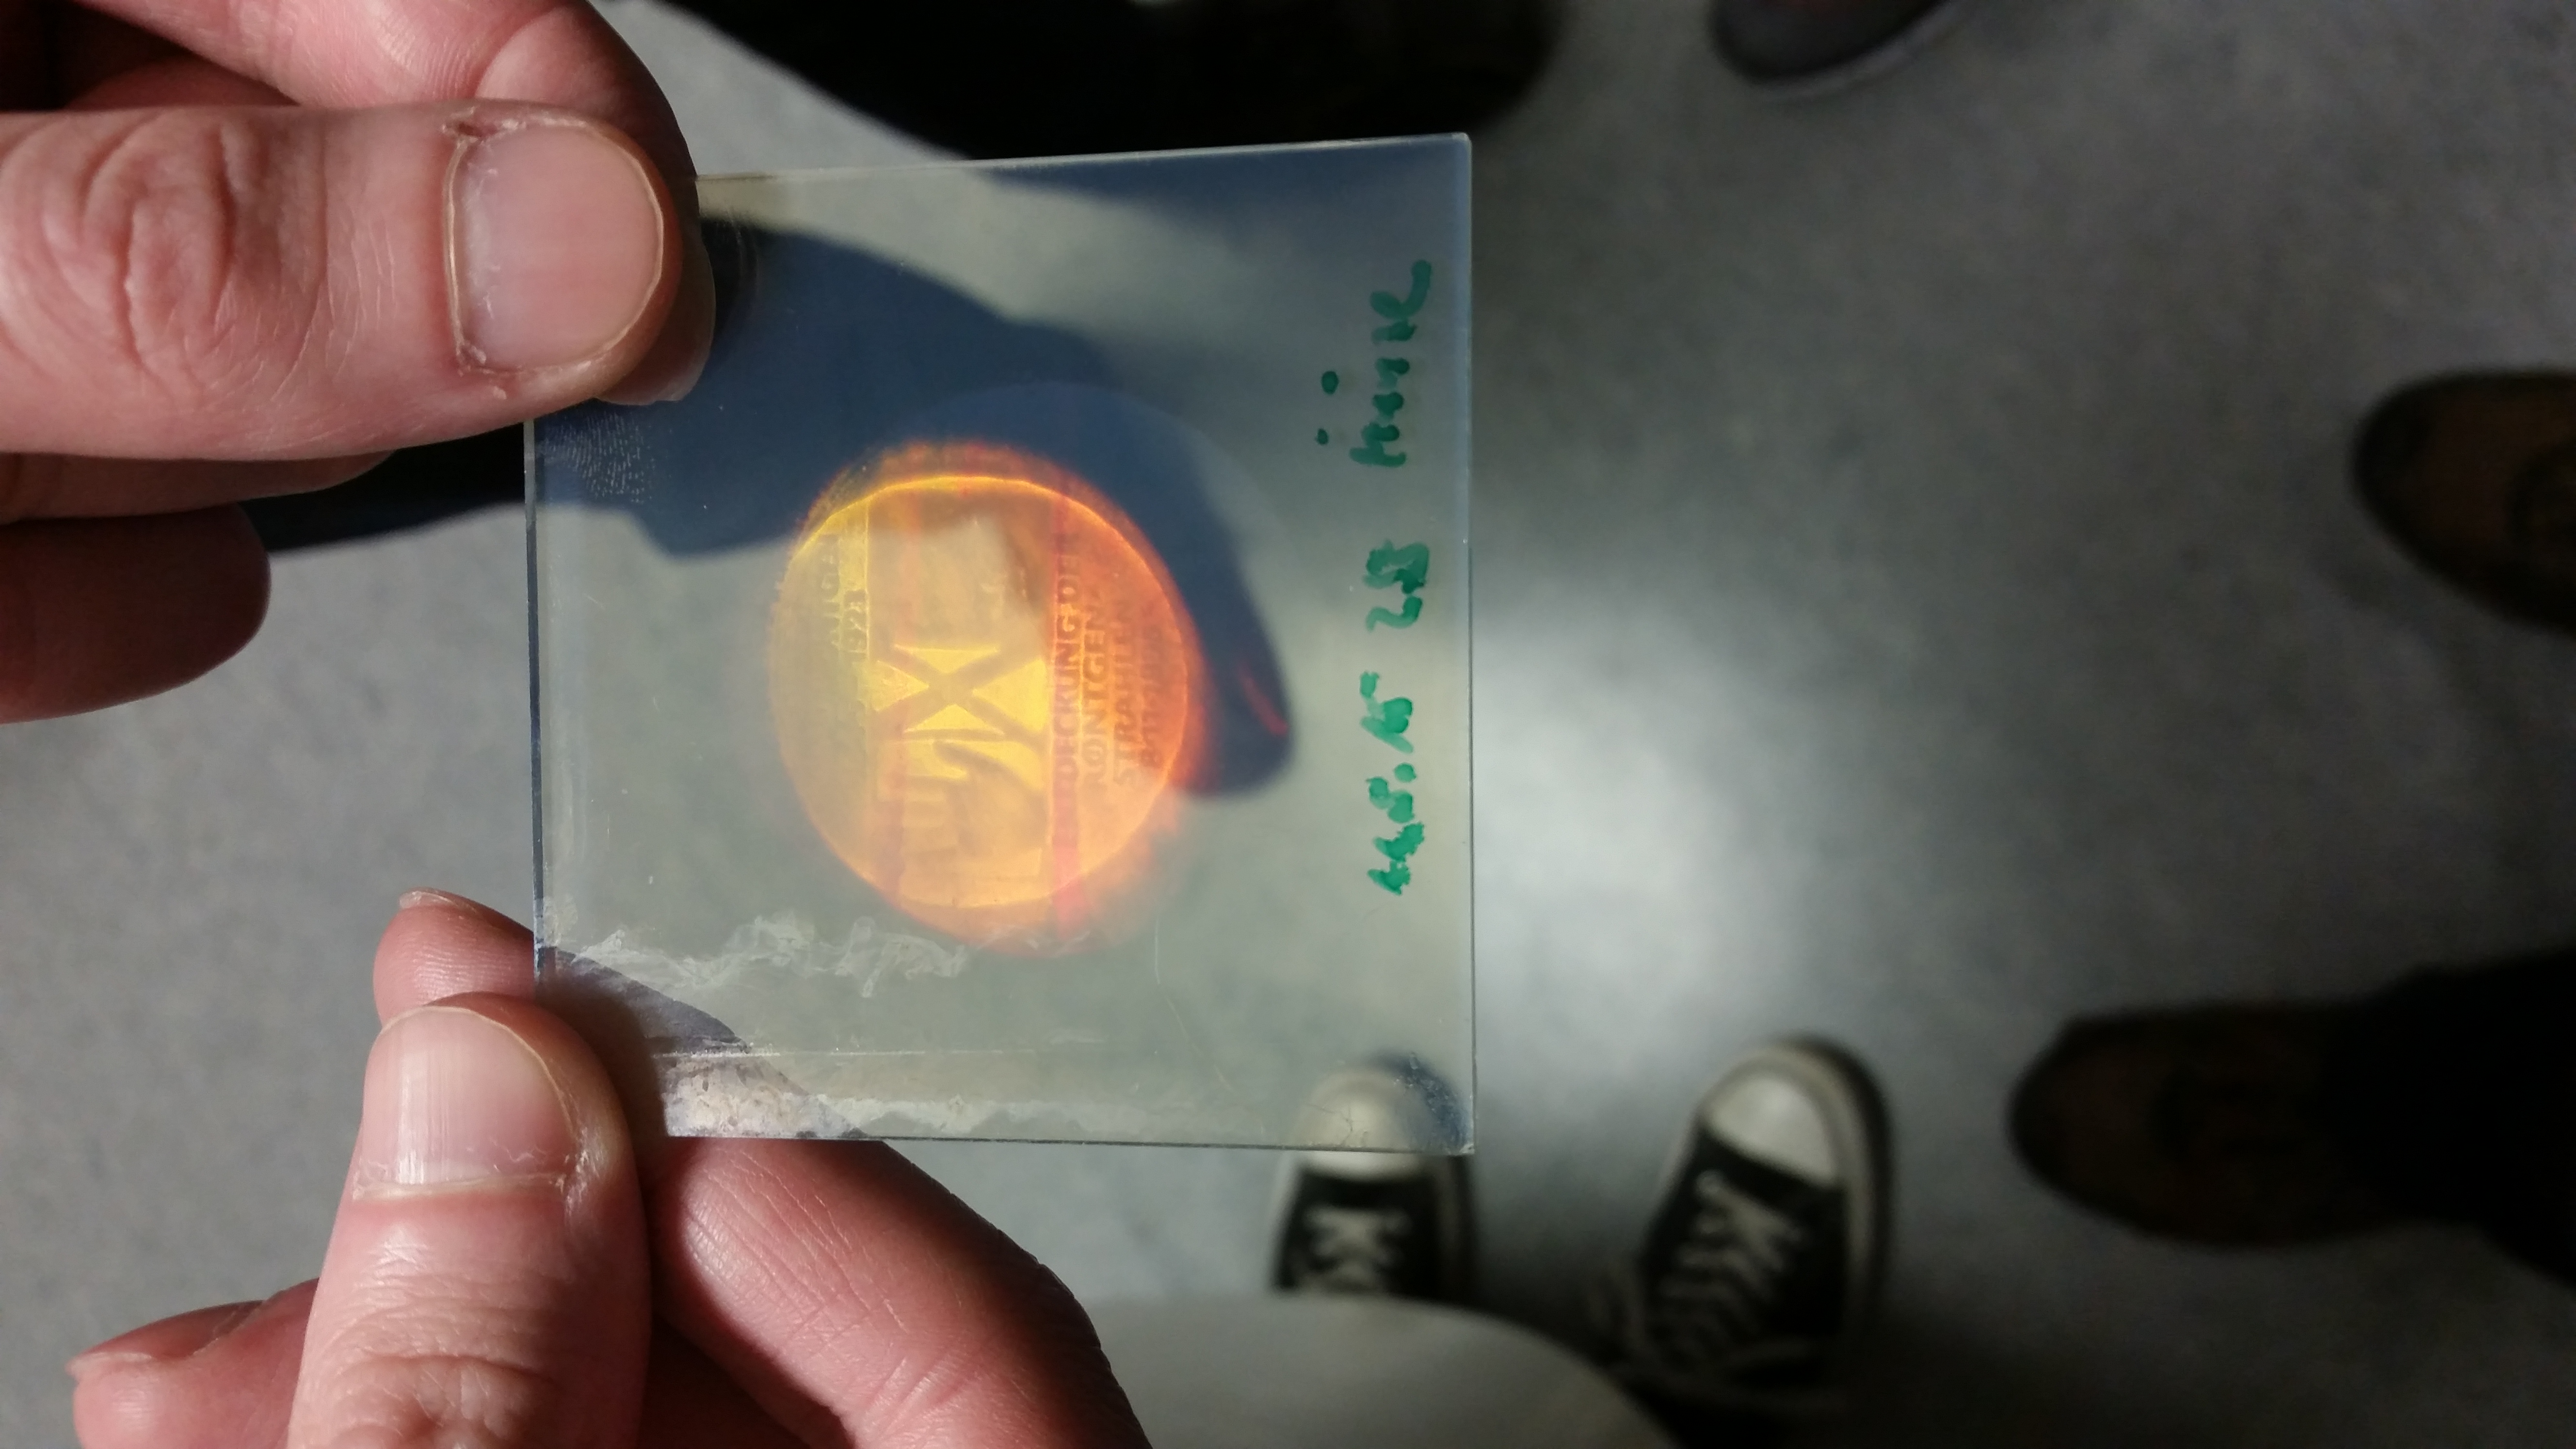
\includegraphics[width=\textwidth]{img/Hologramm-1-Tageslicht.jpg}
    \caption{Hologramm der Münze}
    \label{fig:gedenkholo}
  \end{subfigure}
  \quad%
  \begin{subfigure}[h]{0.3\textwidth}
    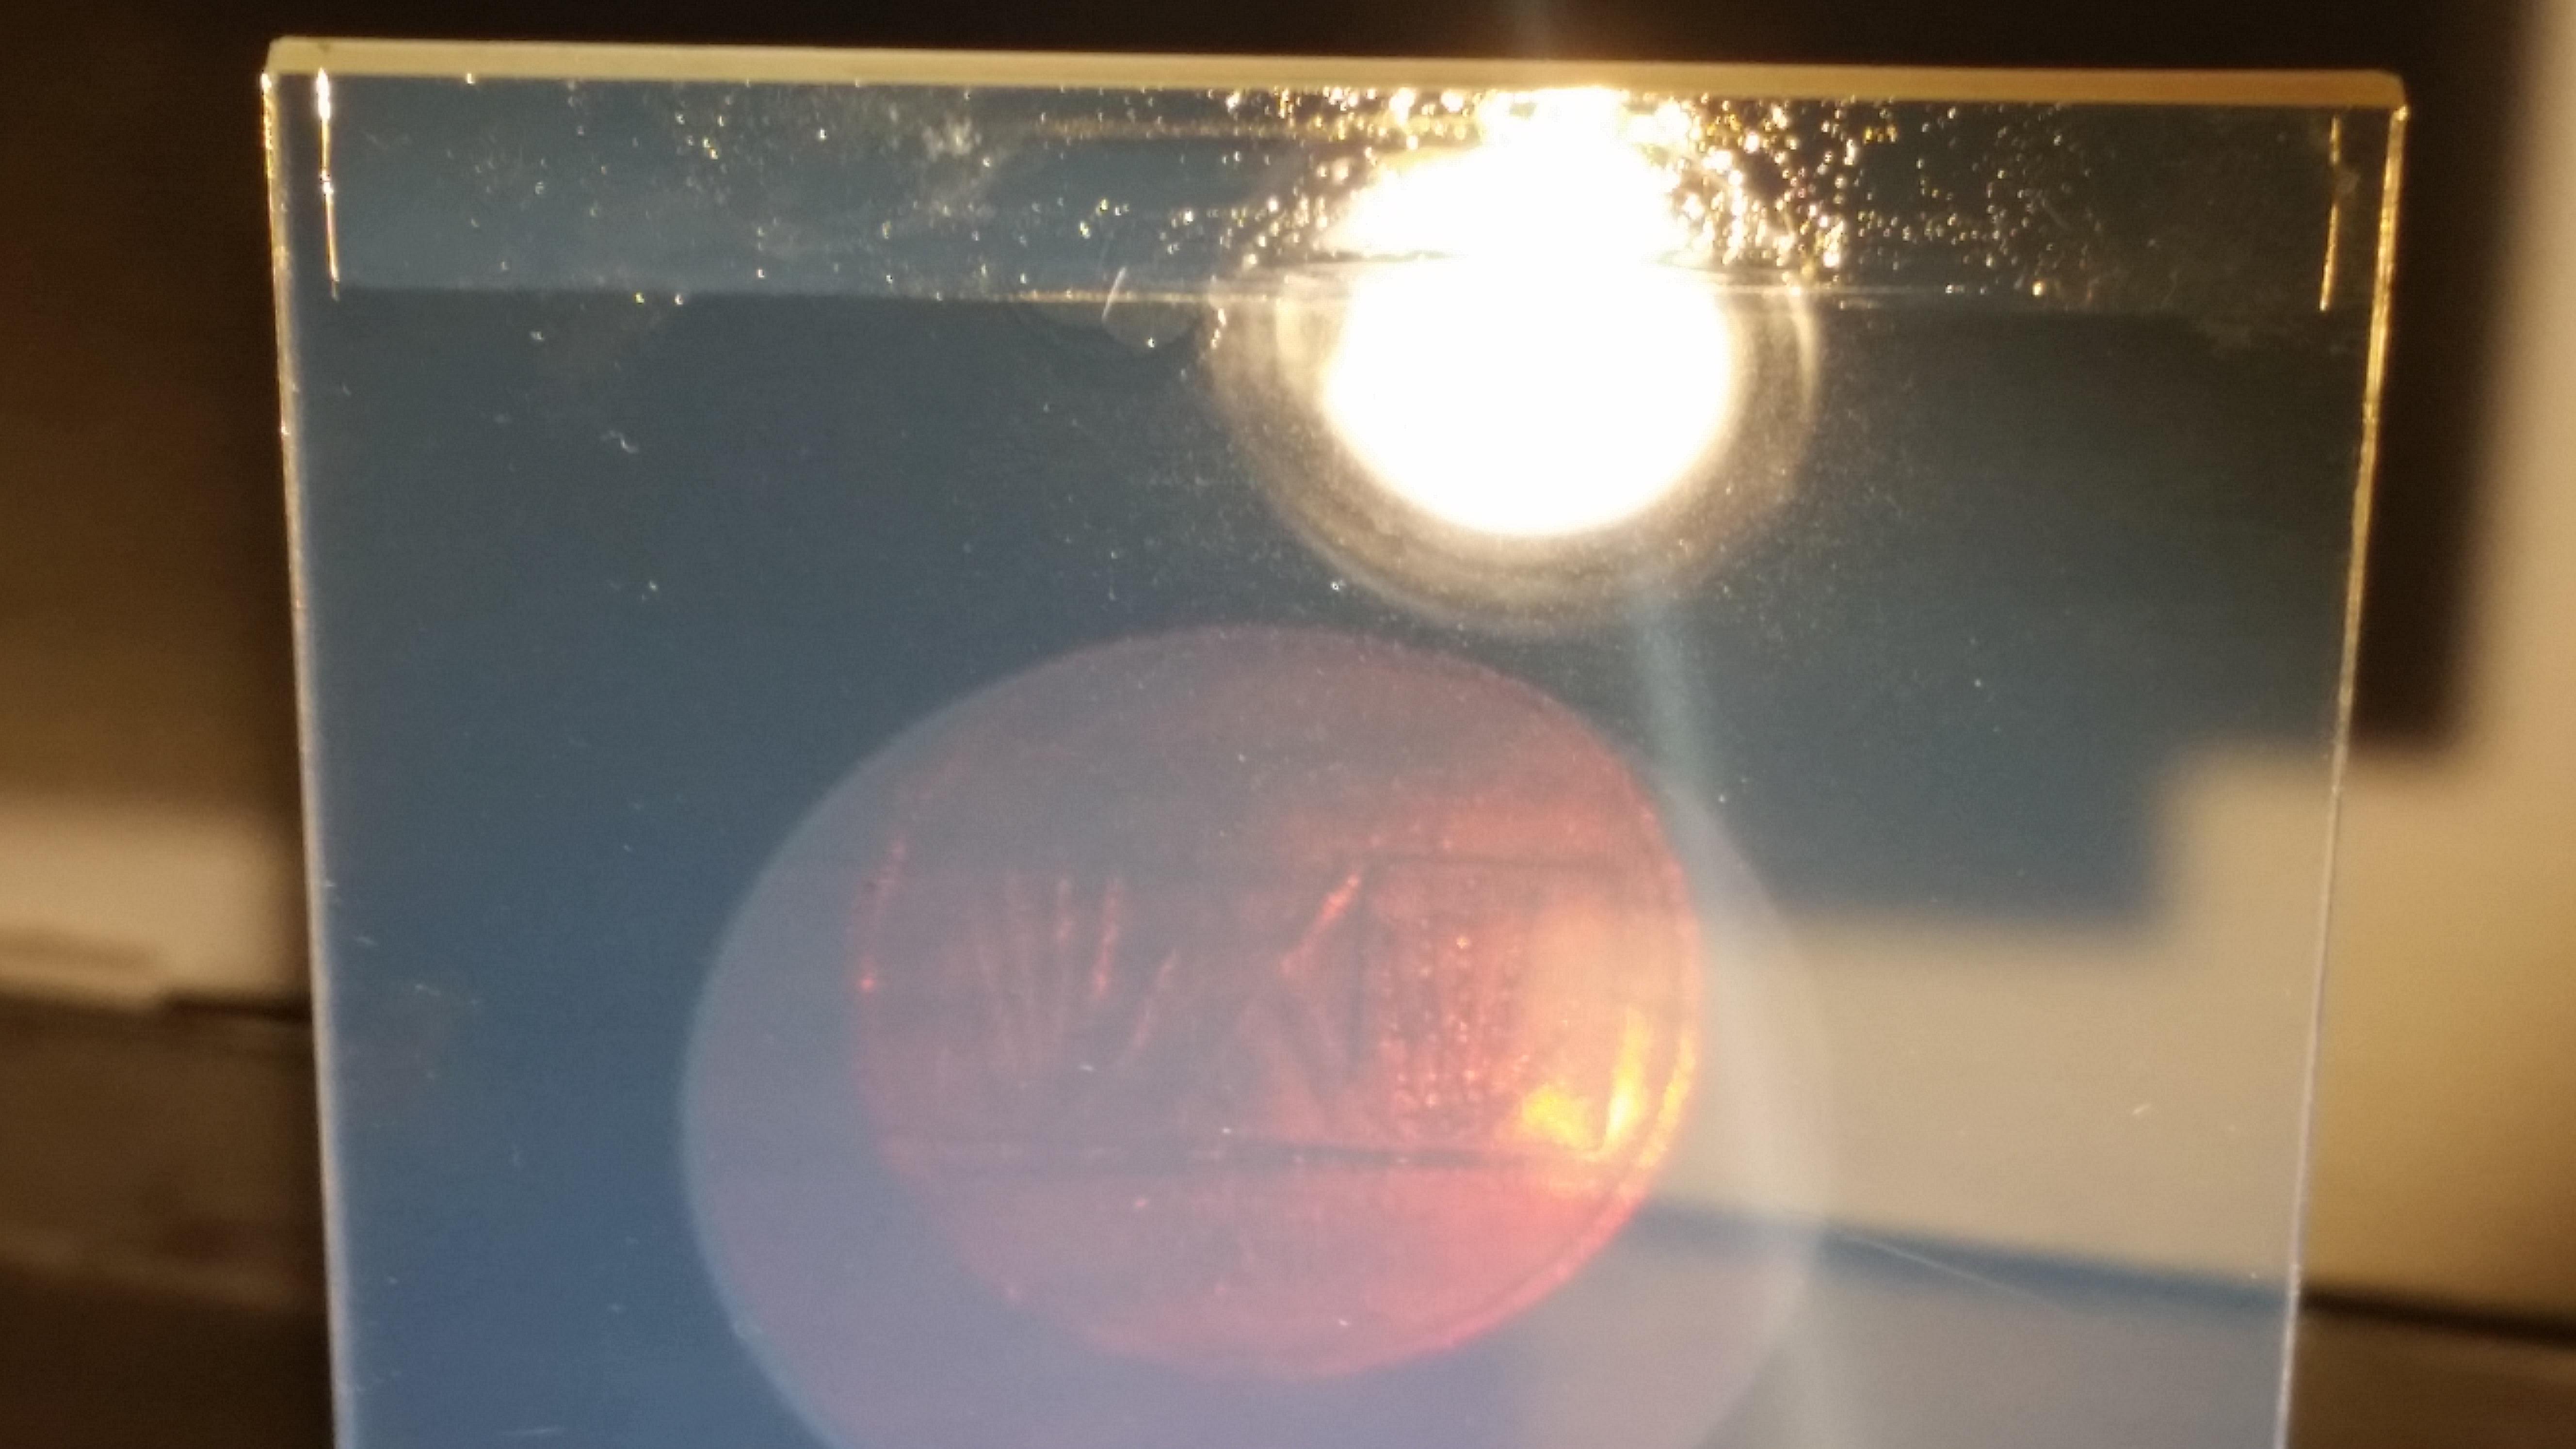
\includegraphics[width=\textwidth]{img/Hologramm-2-Kopie}
    \caption{Hologramm des Hologramms der Münze}
    \label{fig:gedenkholokopie}
  \end{subfigure}
  \caption{Objekt, Hologramm und Kopie des Hologramms. Mit dem bloßen Auge waren
  beide Hologramme noch besser zu erkennen, sogar die Schrift der Münze war leserlich.}\label{fig:genkhologramme}
\end{figure}

\color{blue}
Bei Betrachtung des Hologramms unter verschiedenen Winkeln fallen zwei Dinge auf. Wenn man es von der anderen Seite, also der Objektseite, anschaut, erscheint es vergrößert und spiegelverkehrt. Verantwortlich dafür ist die Tatsache, dass jeder Punkt des reellen Bildes den gleichen Abstand zum Hologramm besitzt wie der entsprechende Punkt des virtuellen Punktes. Das bedeutet, im rellen Bild erscheinen die am ursprünglichen Objekt entfernten Punkte weiter vorne im Bild zu sein und die vorderen Punkte scheinen weiter entfernt zu sein. Diese Umkehrung nennt man Pseudoskopie. Das virtuelle Bild zeigt die wahren Abstände, man nennt es deshalb auch orthoskopisch.

Schaut man von oben schräg auf das Hologramm und lässt Licht von unten schräg auf die gleiche Seite einfallen, beobachtet man eine Farbveränderung. Ab einem gewissen Winkel ist die Bragg-Reflexion dafür verantwortlich, dass vermehrt grünes Licht reflektiert wird und für rotes, längerwelliges Licht destruktive Interferenz auftritt.
\color{black}

\chapter{Fazit}

Abschließend lässt sich feststellen, dass sowohl die Anfertigung eines Hologramms hervorragend gelungen ist, was eindrucksvoll am Hologramm des Hologramms ersichtlich wird. Offensichtlich ist die Holografie mit den zur Verfügung stehenden Materialien sehr gut möglich. Außerdem war es auch möglich mittels der Messwerte die Theorie des holografischen Abbildungsgesetzes zu bestätigen, d.h. auch quantitativ sind die durchgeführten Messungen zielführend. Die Grundlagen der Holografie wie auch die Vorbereitung dafür (Justage des Raumfilters, Bereitstellen der Photochemikalien) werden in diesem Versuch auf interessante Weise dargelegt.

%ENDE INHALT
\cleardoublepage{}
% Eintrag fürs Inhaltsverzeichnis
\newpage
\begin{thebibliography}{100}
  \bibitem{anleitung} Versuchsanleitung zum Versuch Holographie, heruntergeladen am 09.05.2015 von der Homepage des IAP der TU Darmstadt
  \bibitem{blackbodycoherence} The coherence length of black-body
radiation by Axel Donges, 1998: \url{http://hank.uoregon.edu/teaching-modules/Broadband-Interferometer/BBcoherence.pdf}
  \bibitem{boltzmann} Abteilung theoretische Chemie der Goethe-Universität
    Frankfurt von Prof. J. Wachtveitl: \url{http://www.theochem.uni-frankfurt.de/femtochem/lectures/PC2_Sem/Handouts-PCII-WS-12-13/Zotko_Maxwell-Boltzmann%20Verteilung.pdf}
\end{thebibliography}
\end{document}

%%% Local Variables:
%%% mode: latex
%%% TeX-master: t
%%% End:
